\section{Overview}

\begin{figure}
  \centering
  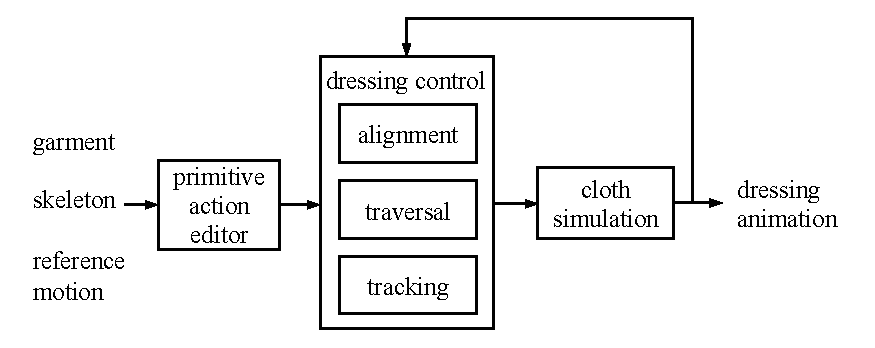
\includegraphics[width=3.3in]{images/overview}
  \caption{The overview of our system.}
  \label{fig:overview}
\end{figure}

\begin{table}
  \centering
  \begin{tabular}{|l|l|}
    \hline
    Action & Description \\
    \hline
    Grip(RH, $\vc{f}_{1}$) & Grip the colar feature $\vc{f}_1$  with the right hand.\\
    Track($\hat{\vc{q}}(t)$, $T_1$) & Track the reference motion $\hat{\vc{q}}$ for $T_1$ seconds.\\
    Align(LH, $\vc{f}_{2}$) & Align the left hand with the armhole $\vc{f}_2$.\\
    Drag(RH, $\{B_i\}$) & Drag the cloth along the left hand $B_1$, the left\\
    &                      arm $B_2$ and the left shoulder $B_3$.\\
    Release(RH) & Release the cloth from the right hand.\\
    Idle($T_2$) & Idle for $T_2$ seconds.\\
    Track($\hat{\vc{q}}$(t), $T_3$) & Track the reference motion $\hat{\vc{q}}$ for $T_3$ seconds.\\
    Align(RH, $\vc{f}_{3}$) & Align the right hand with the right armhole $\vc{f}_3$.\\
    Stretch(RH) & Stretching the right hand into the sleeve.\\
    Track($\hat{\vc{q}}$(t), $T_4$) & Track the reference motion $\hat{\vc{q}}$ for $T_4$ seconds. \\
    \hline
  \end{tabular}
  \caption{An example action queue for dressing the upper body of a character with a jacket.}
  \label{table:actionQueue}
\end{table}


We have designed a system that allows a virtual human character to put on various types of garments. Our system consists of three main components: action queue, dressing control the cloth simulation.
At each step, our system fetches an action from the queue,
executes its corresponding dressing controllers and simulates the physics of the cloth. Figure \ref{fig:overview} illustrates the main components of our system. 
Given a piece of garment, a character and a reference dressing motion, our system allows a user to decompose the entire
dressing sequence into a queue of high level actions. For example, putting an arm into a sleeve involves \emph{aligning} the hand with the armhole and
\emph{dragging} the cloth from the wrist to the shoulder. 
Table~\ref{table:actionQueue} shows complete action queue for putting on a jacket.
For each action, we design kinematic dressing controllers that determine desired end effector positions based on the current cloth states, solves IK problems for full body poses and plans a collision-free joint path to fulfill the action. 





